\documentclass[preprint2]{aastex}

%% preprint2 produces a double-column, single-spaced document:

%% \documentclass[preprint2]{aastex}

%% Sometimes a paper's abstract is too long to fit on the
%% title page in preprint2 mode. When that is the case,
%% use the longabstract style option.

%% \documentclass[preprint2,longabstract]{aastex}

%% If you want to create your own macros, you can do so
%% using \newcommand. Your macros should appear before
%% the \begin{document} command.
%%
%% If you are submitting to a journal that translates manuscripts
%% into SGML, you need to follow certain guidelines when preparing
%% your macros. See the AASTeX v5.x Author Guide
%% for information.

\usepackage{graphicx}
%\usepackage{caption}
%\usepackage{subcaption}
\usepackage{subfigure}
\usepackage{amsmath,amssymb}
\bibliographystyle{apj}
\usepackage{natbib}
\usepackage{textcomp}
\usepackage{lineno}
\newcommand{\tapp}{\raisebox{0.5ex}{\texttildelow}}
\newcommand{\vdag}{(v)^\dagger}
\newcommand{\myemail}{}
\newcommand{\pflux}{~cm$^{-2}$ s$^{-1}$}
\newcommand{\lsi}{LS~I~+61$^{\circ}$~303}
\newcommand{\gev}{\,GeV}
\newcommand{\tev}{\,TeV}
\linenumbers
%% You can insert a short comment on the title page using the command below.


%% If you wish, you may supply running head information, although
%% this information may be modified by the editorial offices.
%% The left head contains a list of authors,
%% usually a maximum of three (otherwise use et al.).  The right
%% head is a modified title of up to roughly 44 characters.
%% Running heads will not print in the manuscript style.

\shorttitle{Bright TeV flares from \lsi{}}
\shortauthors{}

%% This is the end of the preamble.  Indicate the beginning of the
%% paper itself with \begin{document}.

\begin{document}

%% LaTeX will automatically break titles if they run longer than
%% one line. However, you may use \\ to force a line break if
%% you desire.

\title{Exceptionally bright TeV flares from the binary \lsi{}}

%% Use \author, \affil, and the \and command to format
%% author and affiliation information.
%% Note that \email has replaced the old \authoremail command
%% from AASTeX v4.0. You can use \email to mark an email address
%% anywhere in the paper, not just in the front matter.
%% As in the title, use \\ to force line breaks.

\author{
S.~Archambault\altaffilmark{1},
A.~Archer\altaffilmark{2},
T.~Aune\altaffilmark{3},
A.~Barnacka\altaffilmark{4},
W.~Benbow\altaffilmark{5},
R.~Bird\altaffilmark{6},
V.~Bugaev\altaffilmark{2},
M.~Cerruti\altaffilmark{5},
X.~Chen\altaffilmark{7,8},
L.~Ciupik\altaffilmark{9},
W.~Cui\altaffilmark{10},
J.~D.~Eisch\altaffilmark{11},
J.~P.~Finley\altaffilmark{10},
H.~Fleischhack\altaffilmark{8},
A.~Flinders\altaffilmark{12},
L.~Fortson\altaffilmark{13},
G.~H.~Gillanders\altaffilmark{14},
S.~Griffin\altaffilmark{1},
J.~Grube\altaffilmark{9},
G.~Gyuk\altaffilmark{9},
M.~H\"{u}tten\altaffilmark{8},
D.~Hanna\altaffilmark{1},
J.~Holder\altaffilmark{15},
P.~Kaaret\altaffilmark{16},
P.~Kar\altaffilmark{12},
M.~Kertzman\altaffilmark{17},
Y.~Khassen\altaffilmark{6},
D.~Kieda\altaffilmark{12},
M.~Krause\altaffilmark{8},
F.~Krennrich\altaffilmark{11},
M.~J.~Lang\altaffilmark{14},
K.~Meagher\altaffilmark{18},
P.~Moriarty\altaffilmark{14},
A.~O'Faol\'{a}in de Bhr\'{o}ithe\altaffilmark{8},
R.~A.~Ong\altaffilmark{3},
A.~N.~Otte\altaffilmark{18},
N.~Park\altaffilmark{19},
M.~Pohl\altaffilmark{7,8},
A.~Popkow\altaffilmark{3},
E.~Pueschel\altaffilmark{6},
J.~Quinn\altaffilmark{6},
K.~Ragan\altaffilmark{1},
G.~T.~Richards\altaffilmark{18},
E.~Roache\altaffilmark{5},
G.~H.~Sembroski\altaffilmark{10},
A.~W.~Smith\altaffilmark{20},
I.~Telezhinsky\altaffilmark{7,8},
J.~V.~Tucci\altaffilmark{10},
J.~Tyler\altaffilmark{1},
S.~Vincent\altaffilmark{8},
S.~P.~Wakely\altaffilmark{19},
O.~M.~Weiner\altaffilmark{21}
}

\altaffiltext{1}{Physics Department, McGill University, Montreal, QC H3A 2T8, Canada}
\altaffiltext{2}{Department of Physics, Washington University, St. Louis, MO 63130, USA}
\altaffiltext{3}{Department of Physics and Astronomy, University of California, Los Angeles, CA 90095, USA}
\altaffiltext{4}{Harvard-Smithsonian Center for Astrophysics, 60 Garden Street, Cambridge, MA 02138, USA}
\altaffiltext{5}{Fred Lawrence Whipple Observatory, Harvard-Smithsonian Center for Astrophysics, Amado, AZ 85645, USA}
\altaffiltext{6}{School of Physics, University College Dublin, Belfield, Dublin 4, Ireland}
\altaffiltext{7}{Institute of Physics and Astronomy, University of Potsdam, 14476 Potsdam-Golm, Germany}
\altaffiltext{8}{DESY, Platanenallee 6, 15738 Zeuthen, Germany}
\altaffiltext{9}{Astronomy Department, Adler Planetarium and Astronomy Museum, Chicago, IL 60605, USA}
\altaffiltext{10}{Department of Physics and Astronomy, Purdue University, West Lafayette, IN 47907, USA}
\altaffiltext{11}{Department of Physics and Astronomy, Iowa State University, Ames, IA 50011, USA}
\altaffiltext{12}{Department of Physics and Astronomy, University of Utah, Salt Lake City, UT 84112, USA}
\altaffiltext{13}{School of Physics and Astronomy, University of Minnesota, Minneapolis, MN 55455, USA}
\altaffiltext{14}{School of Physics, National University of Ireland Galway, University Road, Galway, Ireland}
\altaffiltext{15}{Department of Physics and Astronomy and the Bartol Research Institute, University of Delaware, Newark, DE 19716, USA}
\altaffiltext{16}{Department of Physics and Astronomy, University of Iowa, Van Allen Hall, Iowa City, IA 52242, USA}
\altaffiltext{17}{Department of Physics and Astronomy, DePauw University, Greencastle, IN 46135-0037, USA}
\altaffiltext{18}{School of Physics and Center for Relativistic Astrophysics, Georgia Institute of Technology, 837 State Street NW, Atlanta, GA 30332-0430}
\altaffiltext{19}{Enrico Fermi Institute, University of Chicago, Chicago, IL 60637, USA}
\altaffiltext{20}{University of Maryland, College Park / NASA GSFC, College Park, MD 20742, USA}
\altaffiltext{21}{Physics Department, Columbia University, New York, NY 10027, USA}


\begin{abstract}
The TeV binary system \lsi{} is known for its regular, non-thermal emission pattern which traces the orbital period of the compact object in its 26.5 day orbit around its B0 Ve star companion. The system typically presents elevated TeV emission around apastron passage with flux levels between 5 and 15\,\% of the steady flux from the Crab Nebula ($>300$\gev{}). In this article, VERITAS observations of \lsi{} taken in late 2014 are presented, during which bright TeV flares around apastron at flux levels peaking above $30\%$ of the Crab Nebula flux were detected. This is the brightest such activity from this source ever seen in the TeV regime. The strong outbursts have rise and fall times of less than a day. The short timescale of the flares, in conjunction with the observation of 10\tev{} photons from \lsi{} during the flares, provides constraints on the nature and efficiency of the accelerating mechanism in the source.
\end{abstract}


\keywords{binaries: general --- gamma rays: observations --- stars: individual (\lsi{}) --- stars: individual (VER J0240+612)--- X-rays: binaries}

\section{Introduction}

High-mass X-ray binaries (HMXBs) are a class of binary system that consist of a compact object (either a black hole or a neutron star) and a massive stellar companion, and emit in X-rays. The current generation of imaging atmospheric-Cherenkov telescopes (IACTs) has facilitated the study of HMXBs which exhibit TeV emission. The class of TeV binaries is quite sparse, consisting of only a handful of sources: LS 5039 \citep{2005Sci...309..746A}, PSR B1259-63 \citep{2005A&A...442....1A}, \lsi{} \citep{Albert2006}, HESS J0632+057 \citep{2007A&A...469L...1A}, 1FGL J1018.6-5856 \citep{2015arXiv150302711H}, and the newest member of the class, TeV 2032+413 \citep{2015MNRAS.451..581L}. Of these, only the compact objects of PSR B1259-63 and TeV 2032+413 have been firmly identified as pulsars. There is still a large degree of ambiguity concerning the nature of the compact object within the other systems. Consequently, the fundamental mechanism responsible for the TeV emission along with its characteristic variability on the timescale of one orbital period remains uncertain.

% For instance, the presence of a pulsar within a given TeV binary indicates that the emission in the system is generated by the shock formed at the interface between the pulsar and stellar winds. The orbital variability is therefore driven principally by the varying density of the stellar wind that the pulsar encounters in its orbit. In the case of a black hole companion, the emission is driven by an accretion-powered jet.

%Modeling of the emission from these objects has driven a very active field with models falling into both of the above categories (binary pulsar vs microquasar), as well as utilizing both leptonic and hadronic emission scenarios. As more ``direct'' attempts to measure the nature of the systems in question have yet to yield decisive information (for example, constraining the inclination angle of viewing to narrow the compact mass down to rule out a black hole) the way forward appears to be further monitoring of the systems across the spectrum in the hopes of discovering some observational feature that would firmly identify these systems and the basic interacting parts within them. 

The orbital periods of TeV-emitting HMXBs vary from several days (LS 5039) to many years (TeV 2032+413). As the TeV emission varies strongly as a function of the orbital phase, the various sources may only have short windows during which they can be detected and studied in the TeV regime. Of the TeV binaries, \lsi{} is the only known source in the Northern Hemisphere that has a short enough orbital period (26.5 days) to allow for regular study with TeV instruments. 

Located at a distance of $\sim2$ kpc \citep{1991AJ....101.2126F}, \lsi{} is composed of a B0 Ve star and a compact object \citep{HandC1981, Casares2005}. The observed multiwavelength emission is variable at all energies and modulated with a period of $P \approx 26.5$ days, believed to be associated with the orbital motion of the binary system \citep{Albert2006, Esposito2007, VERITASLSIDetection, Abdo2009, LiXray, 2015A&A...575L...9M}. Radial velocity measurements show the orbit to be elliptical with eccentricity $e = 0.537\pm0.034$, with periastron occurring around phase $\phi=0.275$, apastron at $\phi=0.775$, superior conjunction at $\phi=0.081$ and inferior conjunction at $\phi=0.313$ \citep{Aragona2009}. The periastron distance between the star and the compact object is estimated at $2.84 \times 10^{12}$\,cm (0.19\,AU) and the apastron distance at $9.57 \times 10^{12}$\,cm (0.64\,AU) \citep{2013A&ARv..21...64D}. However, the inclination of the system is not exactly known but is expected to lie in the range $10^\circ$\,--~$60^\circ$ according to \citet{Casares2005}, leading to some uncertainty in the orbital parameters.

%As a TeV source, \lsi{} has presented puzzling behavior. Initial detections in 2006\,--\,2007 by both the MAGIC \citep{Albert2006} and VERITAS \citep{VERITASLSIDetection} collaborations over many orbital cycles showed the source to be a variably bright TeV source, with emission peaking around apastron passage. Subsequent observations in 2008\,--\,2010 \citep{2011ApJ...738....3A} showed no evidence for emission during these previously detected phases, instead only detecting the source at a lower TeV flux near the periastron passage of a single orbit. However, VERITAS observations taken in November\,--\,December 2011 showed the source to be highly active around apastron again \citep{2013ApJ...779...88A}, similar to the behavior observed in 2006\,--\,2007. Since 2011, observations of \lsi{} by VERITAS have only revealed typical emission levels, i.e., 5\,--\,15\% of the Crab Nebula flux, with emission peaking around apastron.

In this work, we present the results of the VERITAS campaign on \lsi{} in October\,--\,December of 2014. During this time, VERITAS observed historically bright flares from \lsi{} around apastron, with the source exhibiting flux levels a factor of 2\,--\,3 times higher than ever observed.

\section{Observations}
The VERITAS IACT array, located at the base of Mt.\ Hopkins, Arizona (1.3 km a.s.l., 31$^{\circ}40^\prime$\,N, 110$^{\circ}57^\prime$\,W) consists of four 12\,m diameter Davies-Cotton design optical telescopes. VERITAS is sensitive to photons with energies from 85\gev{} to 30\tev{} and has the ability to detect a 1\,\% Crab Nebula source in approximately 25 hours\footnote{\url{http://veritas.sao.arizona.edu/specifications}}. For a full description of the hardware components and analysis methods utilized by VERITAS, see \citet{VERITAS, KiedaVTSUpgrade, VERITASLSIDetection}, and references therein.

In the 2014 season, VERITAS observations of \lsi{} were taken from October 16 (MJD 56946) to  December 12 (MJD 57003), comprising a total of 23.3 hours of quality-selected livetime. These observations sampled three separate orbital periods, covering the orbital phase regions of $\phi = 0.5-0.2$ (see Figure~\ref{f:fluxphase} and Table~\ref{t:fluxphase}). Over the entire set of observations, a total of 449 excess events above an energy threshold of 300\gev{} were detected above background. This is equivalent to a statistical significance of 21 standard deviations \citep[$21\sigma$, calculated using Equation 17 of][]{LiMa}.

\begin{figure}[ht]
\centering
%\subfigure[\label{fig1}]{
%  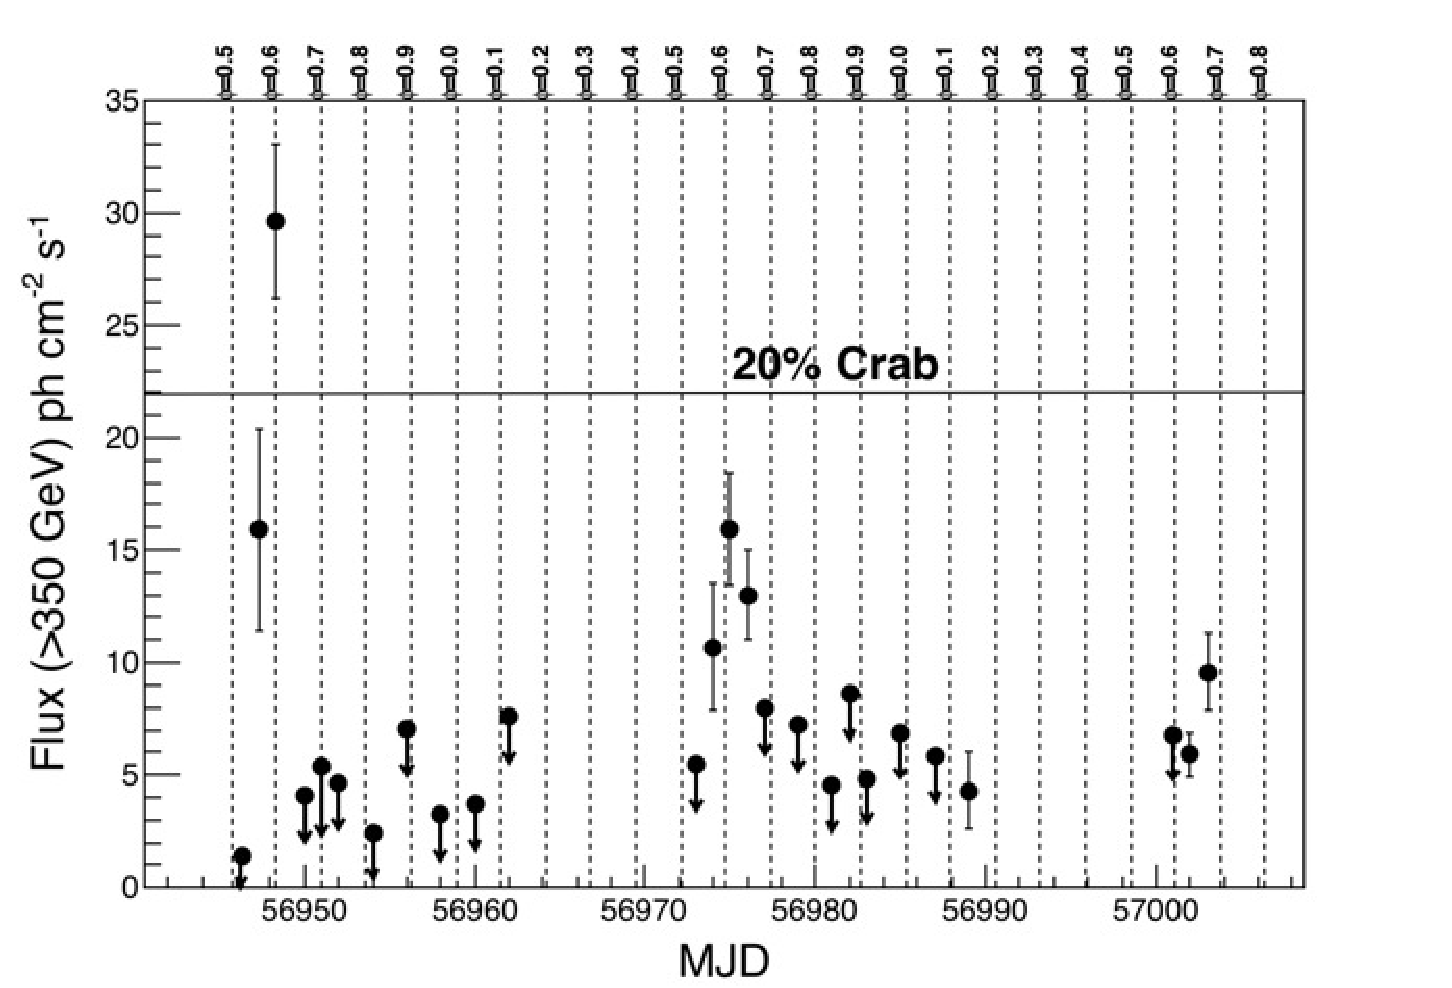
\includegraphics[width=0.5\textwidth]{./figs/Figure1-eps-converted-to.pdf}
%  %\caption{The VERITAS $>$350 GeV light curve of \lsi{} during the 2014 observation season (\textbf{VEGAS}).} 
%  %\label{fig1}
%}
%\subfigure[\label{fig1b}]{
%  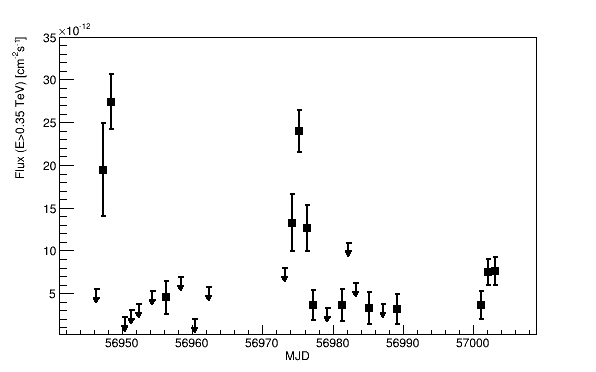
\includegraphics[width=0.5\textwidth]{figs/LSI-mod-lc-days-gt350gev.png}
%  %\caption{The VERITAS $>$350 GeV light curve of \lsi{} during the 2014 observation season (\textbf{ED}).}
%  %\label{fig1b}
%}
\includegraphics[width=0.5\textwidth]{./figs/fluxvphase_300_mod1.pdf}
\caption{Light curve of \lsi{} during the 2014 observation season shown as a function of orbital phase in nightly bins. %from \textbf{VEGAS}~\subref{fig1} and \textbf{ED}~\subref{fig1b}. 
The phase range is shown from 0.45\,--\,0.45 as the VERITAS observations commenced around a phase of $\phi=0.5$ in each orbit. The data for the first orbit (October) are shown with orange circles, while the second orbit (November) is represented by purple diamonds, and the third (December) by blue squares. Flux upper limits at the 99\% confidence level \citep[using the unbounded approach of][]{Rolke} are shown for points with significance $<3\,\sigma$ and are represented by arrows.
}
\label{f:fluxphase}
\end{figure}

\begin{deluxetable}{ccccc}
\tablecolumns{3}
\tablewidth{0pc}
\tablecaption{VERITAS observations of \lsi{} in 2014. The errors quoted on the flux are statistical only. The last column shows the pre-trials significance of the flux difference for each pair of nightly separated fluxes in units of standard deviation. The sections show the division of the data across the three sets of observations taken in October, November, and December, respectively.}
%\tablehead{
%\colhead{MJD} & \colhead{Orbital phase} & \colhead{Flux($>300$\gev{}) [$\times 10^{-11}$\pflux{}]} & \colhead{Duration [mins]} & \colhead{p($F1 > F2$) [$\sigma$]} }
\startdata
\hline\hline
\multicolumn{1}{c}{\vspace{-1.5ex}} & \multicolumn{1}{c}{} & \multicolumn{1}{c}{} & \multicolumn{1}{c}{} & \multicolumn{1}{c}{} \\
\multicolumn{1}{c}{Date} & \multicolumn{1}{c}{Orbital} & \multicolumn{1}{c}{Flux($>300$\gev{})} & \multicolumn{1}{c}{Duration} & \multicolumn{1}{c}{S($F_1 \neq F_2$)} \\
\multicolumn{1}{c}{[MJD]} & \multicolumn{1}{c}{phase ($\phi$)} & \multicolumn{1}{c}{[$\times 10^{-11}$\pflux{}]} & \multicolumn{1}{c}{[mins]} & \multicolumn{1}{c}{[$\sigma$]} \\
\multicolumn{1}{c}{\vspace{-1.5ex}} & \multicolumn{1}{c}{} & \multicolumn{1}{c}{} & \multicolumn{1}{c}{} & \multicolumn{1}{c}{} \\ 
\hline
56946.3\phn & 0.52\phn & $<$0.15\phn\phn\phd\phn\phm{ }\phs\phm{ } & \phn24.5 & $-$ \\  
56947.3\phn & 0.55\phn & \phm{$<$}2.32 $\pm$ 0.54  & \phn21.0 & 5.15 \\
56948.3\phn & 0.60\phn & \phm{$<$}3.20 $\pm$ 0.34 & \phn74.5 & 1.38 \\
56950.0\phn & 0.67\phn & $<$0.47\phn\phn\phd\phn\phm{ }\phs\phm{ } & \phn51.5 & $-$ \\
56951.0\phn & 0.71\phn & $<$0.64\phn\phn\phd\phn\phm{ }\phs\phm{ } & \phn51.1 & 0.94 \\
56952.0\phn & 0.75\phn & $<$0.55\phn\phn\phd\phn\phm{ }\phs\phm{ } & \phn51.0 & 0.56 \\
56954.0\phn & 0.82\phn & $<$0.28\phn\phn\phd\phn\phm{ }\phs\phm{ } & \phn51.1 & $-$ \\
56956.0\phn & 0.90\phn & $<$0.86\phn\phn\phd\phn\phm{ }\phs\phm{ } & \phn51.5 & $-$ \\
56958.0\phn & 0.97\phn & $<$0.38\phn\phn\phd\phn\phm{ }\phs\phm{ } & \phn50.3 & $-$ \\
56960.0\phn & 0.05\phn & $<$0.46\phn\phn\phd\phn\phm{ }\phs\phm{ } & \phn50.7 & $-$ \\
56962.0\phn & 0.12\phn & $<$0.96\phn\phn\phd\phn\phm{ }\phs\phm{ } & \phn50.7 & $-$ \\ \hline
56973.0\phn & 0.54\phn & $<$0.53\phn\phn\phd\phn\phm{ }\phs\phm{ } & \phn25.5 & $-$ \\
56974.0\phn & 0.58\phn & \phm{$<$}1.30 $\pm$ 0.34 & \phn34.4 & 3.63 \\
56975.0\phn & 0.61\phn & \phm{$<$}2.02 $\pm$ 0.22 & 111.3 & 1.80\\
56976.0\phn & 0.65\phn & \phm{$<$}1.55 $\pm$ 0.25 & \phn65.4 & 1.42 \\
56977.0\phn & 0.69\phn & $<$0.94\phn\phn\phd\phn\phm{ }\phs\phm{ } & \phn54.5 & 3.74 \\
56979.0\phn & 0.76\phn & $<$0.85\phn\phn\phd\phn\phm{ }\phs\phm{ } & \phn25.7 & $-$ \\
56981.0\phn & 0.84\phn & $<$0.53\phn\phn\phd\phn\phm{ }\phs\phm{ } & \phn51.3 & $-$ \\
56982.0\phn & 0.88\phn & $<$1.02\phn\phn\phd\phn\phm{ }\phs\phm{ } & \phn25.7 & 0.57 \\
56983.0\phn & 0.92\phn & $<$0.58\phn\phn\phd\phn\phm{ }\phs\phm{ } & \phn33.4 & 0.62 \\
56985.0\phn & 0.99\phn & $<$0.82\phn\phn\phd\phn\phm{ }\phs\phm{ } & \phn48.8 & $-$ \\
56987.0\phn & 0.06\phn & $<$0.69\phn\phn\phd\phn\phm{ }\phs\phm{ } & \phn51.9 & $-$ \\
56989.0\phn & 0.14\phn & $<$1.13\phn\phn\phd\phn\phm{ }\phs\phm{ } & \phn51.6 & $-$ \\ \hline
57001.0\phn & 0.59\phn & $<$0.66\phn\phn\phd\phn\phm{ }\phs\phm{ } & \phn64.6 & $-$ \\
57002.0\phn & 0.63\phn & \phm{$<$}0.72 $\pm$ 0.12 & 144.3 & 2.67 \\
57003.0\phn & 0.67\phn & \phm{$<$}1.06 $\pm$ 0.20 & \phn80.2 & 1.48 \\
\enddata
\label{t:fluxphase}
\end{deluxetable}

During the first orbit observed (in October), the source presented the largest of its flares (hereafter ``F1''), beginning on 2014 October 17 (MJD 56947, $\phi = 0.55$). The emission reached a peak flux of $(3.20 \pm 0.34) \times10^{-11}$\pflux{} above 300\gev{} on October 18 (MJD 56948, $\phi=0.60$). This flare reached a peak flux of approximately $30\%$ of the Crab Nebula flux above the same energy threshold, representing the largest flux ever detected from the source. Unfortunately, observations were limited by poor weather conditions the following two nights and only recommenced on October 20 (MJD 56950), by which time the flux from the source had already decreased. During the second orbital passage in November, VERITAS detected another period of elevated flux (``F2'') from the source at similar orbital phases ($\phi = 0.55-0.65$) with peak emission of $(2.02 \pm 0.22) \times10^{-11}$\pflux{} on November 14 (MJD 56975, $\phi=0.61$).

As an initial test to show that the TeV flux is not stable, the light curves of each orbit were fitted with a constant flux model. Both F1 and F2 were found to be inconsistent with this model at the $10\,\sigma$ level. A test for variability on a nightly timescale was then performed over the complete time range of these observations. For each pair of nightly separated fluxes ($F_1, F_2$) with statistical errors ($\sigma_1,\sigma_2$), the absolute value of the difference of the fluxes was calculated and the errors propagated using the usual variance formula. The probability that the two fluxes are not the same (i.e., $F_1 \neq F_2$) was found in terms of the standard deviation by dividing the difference by the error:
\begin{equation}
S(F_1 \neq F_2) = \frac{|F_1 - F_2|}{\sqrt{(\sigma_1^2 + \sigma_2^2)}}.
\end{equation}
The most significant difference was found between the first and second nights of F1, with a pre-trials significance of $5.15\,\sigma$ corresponding to a post-trials significance of $4.66\,\sigma$ when accounting for the 12 pairs of nightly separated observations.
%using the method described in \citet{2013ApJ...779...88A}. A marginal indication of nightly variability at a significance level of $4.7\,\sigma$ post trials (corresponding to $5.14\,\sigma$ pre trials) was found in F1.
Overall, the data are too sparsely sampled to allow a good measure the rise and fall times of the flares. However, the strong statistical indication of nightly variability and the sharp transition from a flux upper limit to a significantly detected flux over the course of 24 hours at the onset of F1 and F2 imply that the rise time of the flares is of the order of less than one day.

%The rise and fall times of the flares were determined by fitting the following function \citep[Equation 7]{2010ApJ...722..520A} to the light curve of each orbit:
%\begin{equation}
%F(t)=F_c + F_0 \left( e^{\frac{t_0 - t}{t_r}} + e^{\frac{t-t_0}{t_f}} \right),
%\end{equation}
%where $F_c$ is an assumed constant level underlying the flare, $F_0$ is a measure of the amplitude of the flare, $t_0$ is approximately the time of the peak of the flare, and $t_r$ and $t_f$ are the rise and fall time, respectively. The parameter $t_0$ is fixed to the MJD of the observed peak during the fit. The fit to the first orbit has poor fit probability of $P = 3 \times 10^{-7}$ ($\chi^2/\mbox{NDF} = 43.6/7$). %Nevertheless, the rise and fall times of F1 are found to be $0.39 \pm 0.07$ days and $0.37 \pm 0.23$ days, respectively. 
%The second orbit is well fit by this function, with a fit probability of $0.1$ ($\chi^2/\mbox{NDF} = 13.1/8$), possibly due to the better data sampling throughout this flare. The rise and fall times of F2 are found to be $0.65 \pm 0.13$ days and $0.83 \pm 0.12$ days, respectively. The flares were also fitted with a piecewise-defined exponential function of the form
%\begin{equation}
%F(t)=
%\begin{cases}
%F_0 e^{-\frac{|t-t_0|}{t_r}}, & t< t_0 \\
%F_0 e^{-\frac{|t-t_0|}{t_f}}, & t\geq t_0
%\end{cases}
%.
%\end{equation}
% However, poor fit probabilities of $10^{-7}$ and $3 \times 10^{-19}$ were obtained for F1 and F2, respectively. %The rapid increase in flux at the onset of F1 implies flux doubling timescales of less than a day.

Follow-up observations conducted by VERITAS during the next month (December) covered the orbital phases of $\phi=0.59-0.67$ and detected the source at a lower flux level. The previous flares in 2014 were detected at $\phi \simeq 0.60$, but during this cycle the source reached only $(0.72 \pm 0.12) \times10^{-11}$\pflux{} at a comparable orbital phase on December 11 (MJD 57002, $\phi=0.63$). The peak emission of this cycle occurred on the following night at an orbital phase of $\phi=0.67$. The light curve of this orbit was also fitted with a constant flux model and was found to be consistent within $\sim3\,\sigma$. The observations during this month seem to exclude the type of peaked flaring behavior seen around the orbital phase $\phi \simeq 0.60$ in the previous two orbital cycles, indicating some orbit-to-orbit variations in the source.

%As seen in Figure~\ref{f:fig1}, this flare is rather sharply defined: only one night before the flare began, the source was in a quescient state with a $99\%$ confidence upper limit of emission of $1.4 \times10^{-11}$\pflux{} ($>$350 GeV). \textbf{This short variability fast confirms the result of \citep{2013ApJ...779...88A}.}

The average differential photon spectrum from all observations of \lsi{} during the 2014 observing season is well fit with a power law of the form
\begin{equation}
\frac{dN}{dE} = N_0 \left( \frac{E}{1\mbox{\tev{}}} \right)^{-\Gamma},
\end{equation}
in which $N_0$ is the normalization at the pivot energy of 1\tev{}, and $\Gamma$ is the spectral index. The measured parameters are consistent with past observations. Differential photon spectra were also extracted from F1 (October 17\,--\,18) and F2 (November 13\,--\,15) and show a similar spectral shape, albeit with a higher normalization constant. No spectral variability is detected within the statistical errors. The parameters from the spectral fits are given in Table~\ref{t:specfits}. An uncertainty on the energy scale of 15\,--\,25\% results in a systematic uncertainty of $\sim20\%$ on the flux normalization and $\sim40\%$ on the integral flux, assuming a spectral index of 2.34. The systematic uncertainty on the spectral index is estimated at $\sim 0.3$, accounting for uncertainties on the collection efficiency, sky brightness, analysis cuts and simulation model. All spectra are shown in Figure~\ref{spec} along with previous spectral measurements \citep{VERITASLSIDetection,Aleksic} for comparison.

\begin{deluxetable}{ccc}
\tablecolumns{3}
\tablewidth{0pc}
\tablecaption{Spectral parameters of the power law fits to the observations of \lsi{} in the energy range 0.3\,--\,20\tev{}.}
\tablehead{
\colhead{Observations} & \colhead{Normalization [$\times 10^{-12}$ cm$^{-2}$ s$^{-1}$ TeV$^{-1}$]} & \colhead{Spectral index} }
\startdata
All (average) & $1.8 \pm 0.1_{\mathrm{stat}} \pm 0.4_{\mathrm{sys}}$ & $2.34 \pm 0.07_{\mathrm{stat}} \pm 0.3_{\mathrm{sys}}$ \\
F1 (Oct 17\,--\,18) & $8.6 \pm 1.0_{\mathrm{stat}} \pm 1.7_{\mathrm{sys}}$ & $2.24 \pm 0.12_{\mathrm{stat}} \pm 0.3_{\mathrm{sys}}$ \\
F2 (Nov 13\,--\,15) & $4.8 \pm 0.4_{\mathrm{stat}} \pm 1.0_{\mathrm{sys}}$ & $2.36 \pm 0.12_{\mathrm{stat}} \pm 0.3_{\mathrm{sys}}$ \\
\enddata
\label{t:specfits}
\end{deluxetable}

The highest energy gamma-ray candidates observed were detected during the peak night of F1 with an energy of $\sim10$\tev{}. %(using a conservative estimate of the energy). 
There are no events in the \textsc{off} region with energies above 4\tev{} on this night, so it is assumed that the contribution of the background at $\sim10$\tev{} is negligible.

\begin{figure}[ht]
\centering
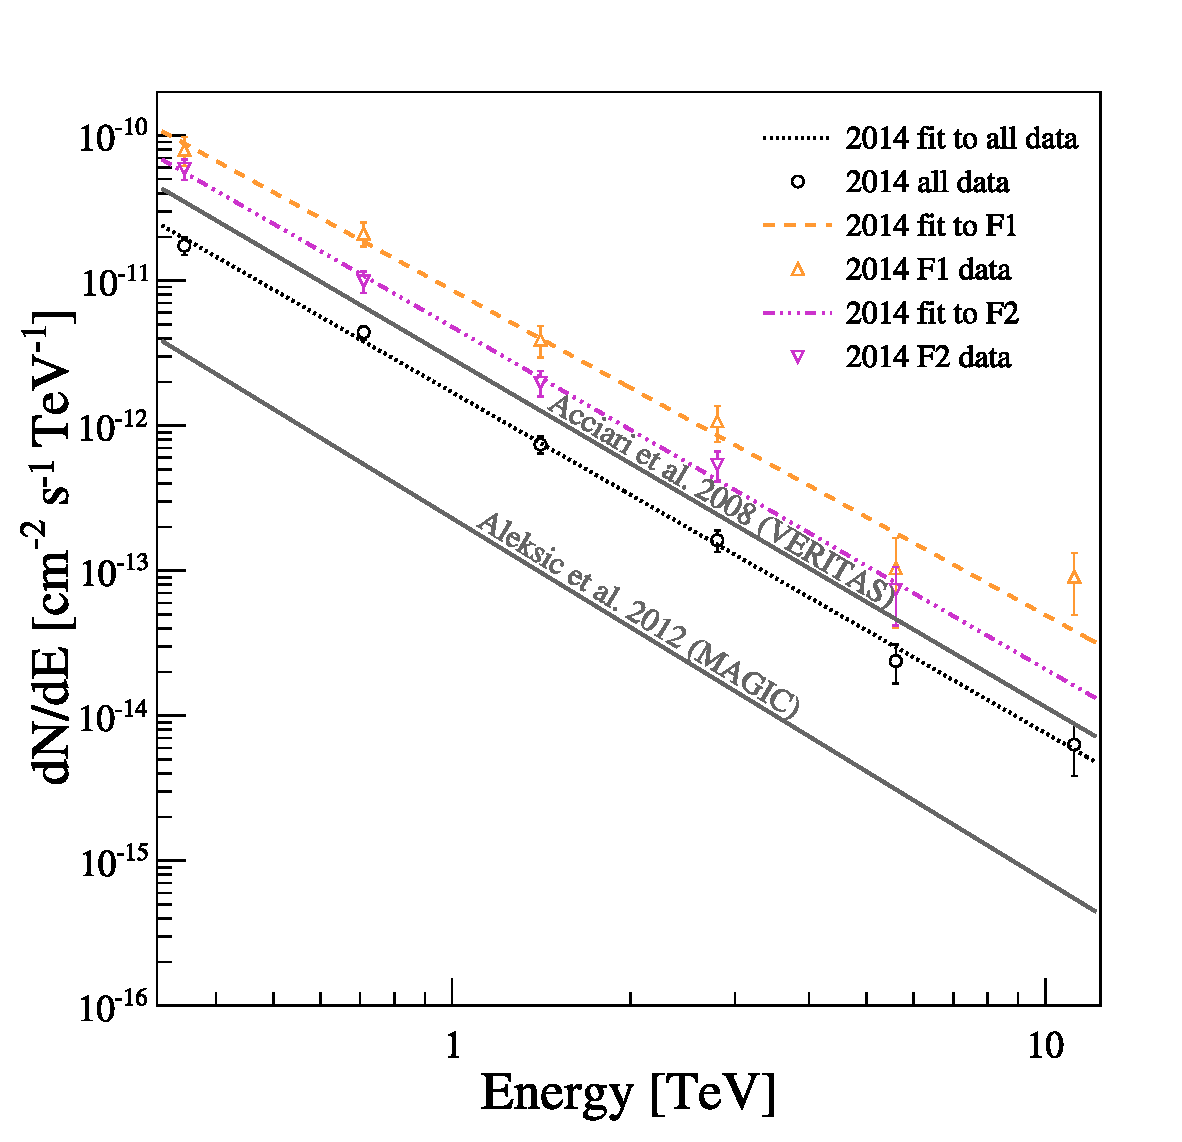
\includegraphics[width=0.5\textwidth]{figs/all_spectra_coloured.pdf}
\caption{Average and flare differential photon spectra of \lsi{} from the VERITAS 2014 observations, shown in comparison with the average spectra from \citet{VERITASLSIDetection} and \citet{Aleksic}.}
\label{spec}
\end{figure}

During these observations, the source was also monitored by the \emph{Fermi}-LAT (0.1\,--\,300\gev{}), the \emph{Swift}-XRT (0.2\,--\,10 keV), and both the RATAN and AMI radio instruments (4/6\,--\,15 GHz). In addition, H$\alpha$ monitoring of the system took place at the Ritter Observatory in Toledo, Ohio (USA). After F2 was detected by VERITAS, an Astronomer's Telegram\footnote{\url{www.astronomerstelegram.org}} \citep{2015VTSATEL} was released, notifying the astronomical community of the historic flux levels and triggering more intense observations by multiwavelength partners, as well as additional observations with the MAGIC TeV observatory. The results of this multiwavelength campaign are under analysis and will be presented in a future publication. 

\section{Discussion and Conclusion}
The nature of the compact object in\linebreak \lsi{} is not firmly established and, as a result, proposed emission mechanisms for the system cover a range of possibilities. These mechanisms fall into two main categories: microquasar ($\mu$Q) and pulsar binary (PB). In the $\mu$Q scenario, non-thermal particle-acceleration processes occur in the jet of an accreting compact object \citep{Massi2001,Massi2013,2015A&A...575L...9M}, whereas the binary pulsar scenario utilizes the presence of a shocked wind in which particle acceleration is the result of the interaction between the stellar and the pulsar winds \citep{Dhawan2006}. While some versions of both models utilize a hadronic primary population, the  majority of both model types employ leptonic origins for the observed non-thermal emission. In a leptonic scenario, the TeV emission is the result of inverse-Compton (IC) scattering of electrons accelerated in the jet ($\mu$Q) or at the shock front (PB).

\citet{Paredes-Fortuny2014} present a general pulsar wind shock scenario with an inhomogeneous stellar wind in which the B0 Ve star disc is disrupted and fragments. The resulting clumps of the disc fall into the shock region, pushing the shock closer to the pulsar. The reduction in size of the pulsar wind termination shock could allow for increased acceleration efficiency on the timescale of a few hours, depending on the size and density of the disc fragments. Such a scenario could account for the exceptionally bright TeV flares and orbit-to-orbit variations seen in \lsi{}.

Regardless of the primary mechanism of generation, \citet{2008MNRAS.383..467K} provide a prescription to calculate model-independent limits on the magnetic field strength and the efficiency of the accelerator within an IC scenario. %It is assumed that the gamma rays are produced in the system by the IC scattering of stellar photons by TeV electrons. 
Given the temperature $T=2.25\times10^4$\,K \citep{2013A&ARv..21...64D} of the B0 Ve star in \lsi{}, the average energy of the stellar photons is $3kT \approx 6$\,eV, and the IC scattering will take place deep in the Klein-Nishina regime, in which almost all of the electron energy is transferred to the scattered photons. Thus, the presence of $\sim10$\tev{} photons requires electrons with an energy of at least $10$\tev{} in the emitter, as well as forcing the acceleration time to be less than the cooling time. As the photon will not carry all the energy from the electron and there is no evidence of a cutoff in the photon spectrum, an example case of a 20\tev{} electron will be used in this discussion. Following the calculations of \citet{2008MNRAS.383..467K}, the acceleration timescale of the electrons can be expressed as
\begin{equation}
t_{\mbox{\scriptsize{acc}}} = \eta_{\mbox{\scriptsize{acc}}} r_{\mbox{\scriptsize{L}}} c^{-1} \approx 0.1 \eta_{\mbox{\scriptsize{acc}}} \left( \frac{E}{1\mbox{\,TeV}} \right) \left( \frac{B}{1\mbox{\,G}} \right)^{-1} \mbox{\,s},
\label{taccel}
\end{equation}
where $r_{\mbox{\scriptsize{L}}}$ is the Larmor radius of the electron, $\left( \frac{E}{1\mbox{\,\scriptsize TeV}} \right)$ is the energy of the electron in units of TeV, $\left( \frac{B}{1\mbox{\,\scriptsize G}} \right)$ is the magnetic field strength in units of Gauss, and $\eta_{\mbox{\scriptsize{acc}}} > 1$ is a parameter describing the efficiency of the accelerator (in general $\eta_{\mbox{\scriptsize{acc}}} \gg 1$). The characteristic cooling time of electrons in the Klein-Nishina regime is given by
\begin{equation}
t_{\mbox{\scriptsize{KN}}} \approx 10^3 \left( \frac{d}{10^{13}\mbox{\,cm}} \right)^2 \left( \frac{E}{1\mbox{\,TeV}} \right)^{0.7} \mbox{\,s},
\end{equation}
where $\left( \frac{d}{10^{13}\mbox{\,\scriptsize cm}} \right)$ is the distance between the emitter and the optical star in units of $10^{13}$\,cm, and the synchrotron cooling time is 
\begin{equation}
t_{\mbox{\scriptsize{sy}}} \approx 4\times10^2 \left( \frac{B}{1\mbox{\,G}} \right)^{-2} \left( \frac{E}{1\mbox{\,TeV}} \right)^{-1} \mbox{\,s}.
\end{equation}
The relation $t_{\mbox{\scriptsize{KN}}} < t_{\mbox{\scriptsize{sy}}}$ can also be set due to the fact that IC losses in the Klein-Nishina regime allow for the hard electron spectra (harder than $2$) necessary to produce hard gamma-ray spectral indices (from $2$ to $2.5$). Thus, the magnetic field in the emitter is constrained by the relation
\begin{equation}
{B < 0.6 \left( \frac{d}{10^{13}\mbox{\,cm}} \right)^{-1} \left( \frac{E}{1\mbox{\,TeV}} \right)^{-0.85} \,\mbox{\,G}}.
\end{equation}
Using $ \left( \frac{E}{1\mbox{\,\scriptsize TeV}} \right) = 20$ gives a value of %$B \lesssim 0.2$\,G at periastron and 
$B \lesssim 0.05$\,G at apastron (close to the position in the orbit at which the flares were detected), assuming that the emitter is located close to the compact object.

A fundamental condition is that the Larmor radius of the electrons must be less than the linear size of the emitter. The distance between the optical star and the location of the emitter can be taken as an upper limit on the extent of the emitting region. As before, it is assumed that the emitter is located close to the compact object, so the distance between the compact object and the emitter is used as an estimate of the linear size of the emitter. Rearranging Equation~\ref{taccel} and including this condition on $r_{\mbox{\scriptsize{L}}}$ yields
\begin{equation}
B > 3 \times 10^{-3} \left( \frac{E}{1\mbox{\,TeV}} \right) \left( \frac{d}{10^{12}\mbox{\,cm}} \right)^{-1}.
\label{rl<d}
\end{equation}
This gives a value of %$B \gtrsim 2 \times 10^{-2} \,\mbox{\,G}$ at periastron and 
$B \gtrsim 6 \times 10^{-3} \,\mbox{\,G}$ at apastron.

As the cooling time is dominated by $t_{\mbox{\scriptsize{KN}}}$, the requirement that the acceleration time is less than the cooling time yields the relation $t_{\mbox{\scriptsize{acc}}} < t_{\mbox{\scriptsize{KN}}}$ which gives
\begin{equation}
B > 10^{-4} \left( \frac{d}{10^{13}\mbox{\,cm}} \right)^{-2} \left( \frac{E}{1\mbox{\,TeV}} \right)^{0.3} \eta_{\mbox{\scriptsize{acc}}} \,\mbox{\,G}.
\end{equation}
This expression can be used in conjunction with the lower limit on the magnetic field strength from Equation~\ref{rl<d} in order to place a limit on the acceleration efficiency parameter of $\eta_{\mbox{\scriptsize{acc}}} \lesssim 22$. This value indicates that the emitter must be host to an extremely efficient acceleration process. 

The constraints are strongly dependent on the assumed location of the emitter, which has been taken to be coincident with the compact object in order to derive these limits. If the emitter is located further from the star, the limit on the acceleration efficiency parameter is less constraining, but the upper limit on the magnetic field is reduced. Regardless of the location of the emitter, the simple Klein-Nishina scattering assumed in this discussion implies a very hard synchrotron spectrum in the X-ray band. Photon indices softer than 1.3 in this energy regime \citep{pkaricrc} may challenge this simple scenario, which requires an electron spectral index harder than 2 to produce hard gamma-ray spectral indices.

%This gives values of $B \gtrsim (2.5 \times 10^{-3}) \eta_{\mbox{\scriptsize{acc}}} \,\mbox{\,G}$ at periastron and $B \gtrsim (2.2 \times 10^{-4}) \eta_{\mbox{\scriptsize{acc}}} \,\mbox{\,G}$ at apastron, if the emitter is close to the compact object. Using the lower and upper limits on the magnetic field strength, an upper limit can be placed on the acceleration efficiency parameter of $\eta_{\mbox{\scriptsize{acc}}} \lesssim 120$ at periastron and $\eta_{\mbox{\scriptsize{acc}}} \lesssim 454$ at apastron.

%Figure~\ref{f:tacc} shows the acceleration time $t_{\mbox{\scriptsize{acc}}}$ as a function of the magnetic field strength $B$ for different values of the accelerator efficiency parameter $\eta_{\mbox{\scriptsize{acc}}}$, assuming an electron energy of 10\tev{}. The upper limits on the magnetic field strength at periastron and apastron, which are independent of $\eta_{\mbox{\scriptsize{acc}}}$, are marked. Two areas of the plot are shaded to indicate the allowed regions of the parameter space, corresponding to $t_{\mbox{\scriptsize{acc}}} < 1$\,day, $B < 0.3$\,G, and $\eta_{\mbox{\scriptsize{acc}}} < 120$ at periastron and $B < 0.1$\,G and $\eta_{\mbox{\scriptsize{acc}}} < 454$ at apastron. 
%\begin{figure}[ht]
%\centering
%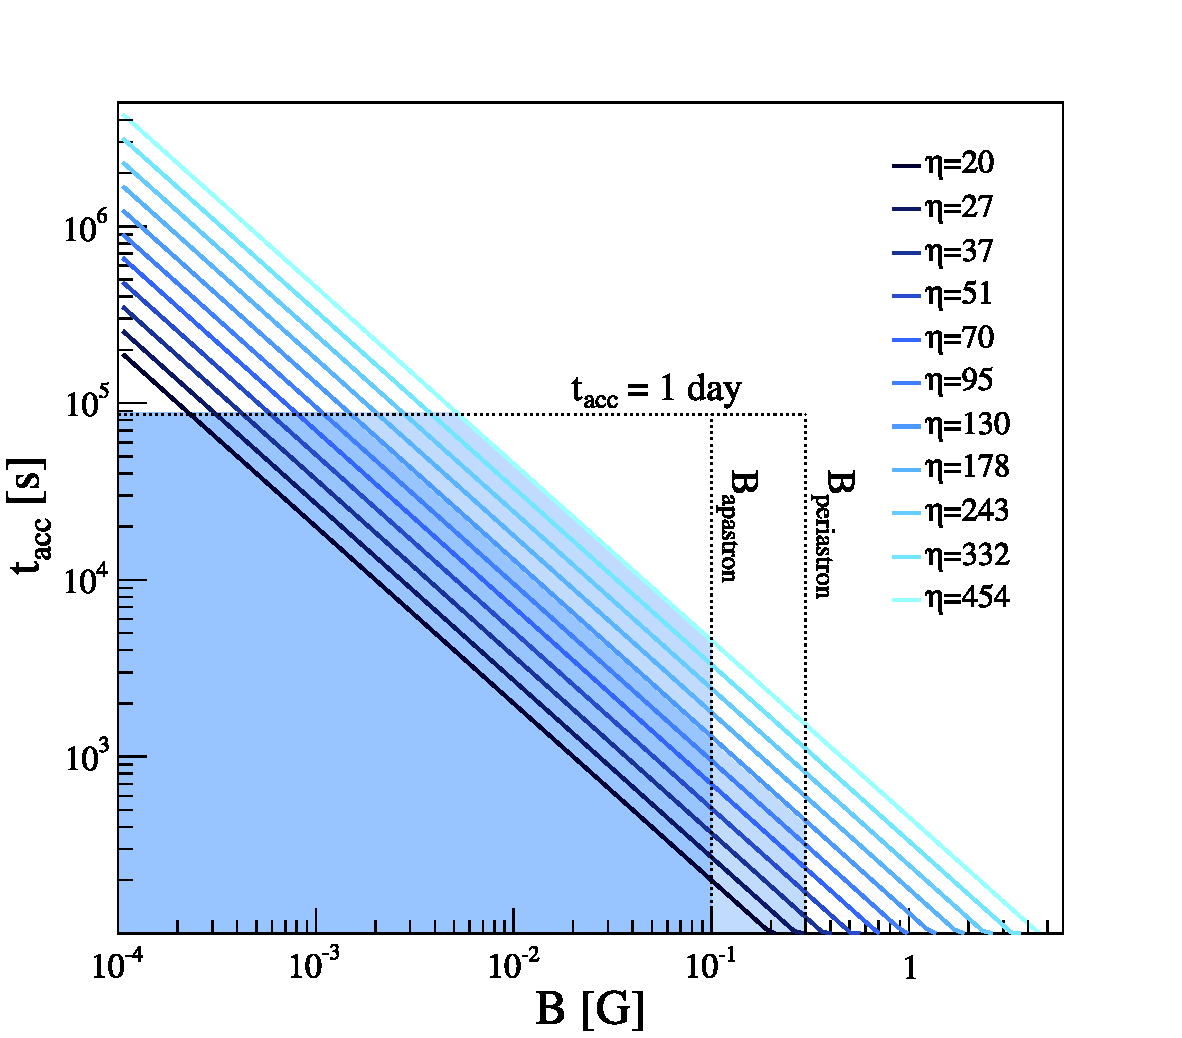
\includegraphics[width=0.5\textwidth]{figs/taccvsB_areas.pdf}
%\caption{Acceleration time $t_{\mbox{\scriptsize{acc}}}$ as a function of the magnetic field strength $B$ for different values of the accelerator efficiency parameter $\eta_{\mbox{\scriptsize{acc}}}$, assuming an electron energy of 10\tev{}. The horizontal dotted line marks an acceleration time of one day, the maximum acceleration time of the 10\tev{} electrons in the system from these observations. The vertical lines labeled $B_{\mbox{\scriptsize{apastron}}}$ and $B_{\mbox{\scriptsize{periastron}}}$ mark the upper limits on the magnetic field strength at apastron and periastron, respectively (these limits are independent of $\eta_{\mbox{\scriptsize{acc}}}$). The shaded regions show the allowed regions of the parameter space for the system at apastron and periastron.}
%\label{f:tacc}
%\end{figure}

% Using these magnetic field values in Equation~\ref{taccel} gives acceleration times in the range $3 \eta_{\mbox{\scriptsize{acc}}}$\,--\,$10 \eta_{\mbox{\scriptsize{acc}}}$. For an efficient (but not extreme) accelerator with $\eta_{\mbox{\scriptsize{acc}}} \approx 50$, this results in acceleration times of a few hundred seconds, much shorter than the observed TeV variability timescales.

The VERITAS observations of the bright flares from \lsi{} in 2014 provide constraints on the physical properties of the system around the acceleration region as well as on the efficiency of the acceleration mechanism. However, these constraints are not enough to hint at either a $\mu$Q or PB system. While the detection of pulsed emission from the source would unambiguously identify the compact object as a pulsar, it is also possible that the dense stellar environment of the source could hinder such a detection. Regardless, further observations of \lsi{} with TeV instruments are necessary to fully understand the varying TeV emission from this source.
\vspace{2ex}

\small{
This research is supported by grants from the U.S. Department of Energy Office of Science, the U.S. National Science Foundation and the Smithsonian Institution, and by NSERC in Canada. We acknowledge the excellent work of the technical support staff at the Fred Lawrence Whipple Observatory and at the collaborating institutions in the construction and operation of the instrument. The VERITAS Collaboration is grateful to Trevor Weekes for his seminal contributions and leadership in the field of VHE gamma-ray astrophysics, which made this study possible. A.\ O'FdB acknowledges support through the Young Investigators Program of the Helmholtz Association. A.W. Smith acknowledges support from the Fermi Cycle 7 Guest Investigator Program, grant number NNH13ZDA001N.
}

\bibliography{refs}

\end{document}

%%
%% End of file `sample.tex'.
